%% LyX 2.4.4 created this file.  For more info, see https://www.lyx.org/.
%% Do not edit unless you really know what you are doing.
\documentclass[english]{article}
\usepackage[T1]{fontenc}
\usepackage[latin9]{inputenc}
\usepackage{amsmath}
\usepackage{amsthm}
\usepackage{amssymb}
\usepackage{geometry}
\geometry{verbose,tmargin=1in,bmargin=1in,lmargin=1in,rmargin=1in}

\makeatletter
%%%%%%%%%%%%%%%%%%%%%%%%%%%%%% User specified LaTeX commands.
\usepackage{fancyhdr}
\usepackage{lastpage}
\pagestyle{fancy}
\usepackage{enumitem}
\usepackage{tikz}
\usetikzlibrary{shapes,snakes}
\usepackage{amsmath,amssymb}
\usepackage{multicol}
% Added by lyx2lyx
\setlength{\parskip}{\smallskipamount}
\setlength{\parindent}{0pt}

\makeatother

\usepackage{babel}
\begin{document}
\lhead{MTH 331(A) Dr.\,James Ashe}
\chead{\textbf{Helpful Results}}
\cfoot{\thepage{}~of~\pageref{LastPage}}
%%
%%\setenumerate[0]{leftmargin=12pt,itemindent=0pt,labelwidth=0pt}
\renewcommand{\labelenumi}{\textbf{\arabic{enumi}.}}


\subsection*{Chapter 9}

\textbf{Geometric Series. }Let $r,a\in\mathbb{R}$. If $|r|<1$, then
${\displaystyle \sum_{k=0}^{\infty}}ar^{k}=\frac{a}{1-r}$. If $|r|\geq1$,
then the series diverges. \vfill

\textbf{Ratio Test. }Let $\sum a_{k}$ be an infinite series with
positive terms and let $r={\displaystyle \lim_{n\rightarrow\infty}\frac{a_{k+1}}{a_{k}}}$.\vspace{-.25cm}
\begin{enumerate}
\item If $0\leq r<1$ then the series converges.
\item If $r>1$ (including $r=\infty$) then the series diverges.
\item If $r=1$ then the test is inconclusive.\vfill
\end{enumerate}
\textbf{Root Test. }Let $\sum a_{k}$ be an infinite series with positive
terms and let $\rho={\displaystyle \lim_{n\rightarrow\infty}\sqrt[k]{a_{k}}}$.\vspace{-.25cm}
\begin{enumerate}
\item If $0\leq\rho<1$ then the series converges.
\item If $\rho>1$ (including $r=\infty$) then the series diverges.
\item If $\rho=1$ then the test is inconclusive.\vfill
\end{enumerate}

\subsection*{Chapter 10}

\textbf{Taylor's Polynomials. }Let $f$ be a function with $f',f'',\dots f^{(n)}$
defined at $a$. The \textbf{\emph{n}}\textbf{th-order Taylor Polynomial
}for $f$ with its \textbf{center }at $a$ denoted $p_{n}$, has the
property that it matches $f$ in value, slope, and all derivatives
up to the \emph{n}th derivative at $a$; that is,
\[
p_{n}(a)=f(a)\mbox{ and }p'_{n}(a)=f'(a),\dots,p_{n}^{(n)}(a)=f^{(n)}(a)\mbox{.}
\]

The \emph{n}th-order Taylor polynomial centered at $a$ is 
\[
p_{n}(x)=f(a)+f'(a)(x-a)+\frac{f''(a)}{2!}(x-a)^{2}+\dots+\frac{f^{(n)}(a)}{n!}(x-a)^{n}\mbox{.}
\]

More compactly, 
\[
p_{n}(x)={\displaystyle \sum_{k=0}^{n}\frac{f^{(k)}(a)}{k!}(x-a)^{k}\mbox{ for }k=0,1,2,\dots,n\mbox{.}}
\]
\vfill

\subsection*{Chapter 11}

\textbf{Slope of a Tangent Line. }Let $f$ be differentiable function
at $\theta_{0}$. The slope of the line tangent to the curve $r=f(\theta)$
at the point $\left(f(\theta),\theta_{0}\right)$ is 
\[
\frac{dy}{dx}=\frac{f'(\theta_{0})\sin\theta_{0}+f(\theta_{0})\cos\theta_{0}}{f'(\theta_{0})\cos\theta_{0}-f(\theta_{0})\sin\theta_{0}}\mbox{,}
\]
 provided the denominator is nonzero at the point. At angles $\theta_{0}$
for which $f(\theta_{0})=0$ and $f'(\theta_{0})\neq0$, the tangent
line is $\theta=\theta_{0}$ with slope $\tan\theta_{0}$.\vfill

\textbf{Area of Regions in Polar Coordinates. }Let \textbf{$R$ }be
the region bounded by the graph of $r=f(\theta)$ and the origin,
between $\theta=\alpha$ and $\theta=\beta$, where $f$ is continuous
and $f(\theta)\geq g(\theta)\geq0$ on $[\alpha,\beta]$. The area
of $R$ is 
\[
{\displaystyle \int_{\alpha}^{\beta}\frac{1}{2}f(\theta)^{2}d\theta}\mbox{.}
\]
\vfill

\begin{multicols}{2}

\subsection*{Helpful formulas}
\begin{enumerate}
\item $\frac{d}{dx}\left(x^{n}\right)=nx^{n-1}$
\item $\frac{d}{dx}\left[f\left(g(x)\right)\right]=f'\left(g(x)\right)\cdot g'(x)$
(Chain rule)
\item $\frac{d}{dx}\left(f(x)g(x)\right)=f'(x)g(x)+f(x)g'(x)$
\item $\frac{d}{dx}e^{x}=e^{x}$
\item $\frac{d}{dx}\sin ax=a\cos ax$
\item $\frac{d}{dx}\cos ax=-a\sin ax$
\item $\int x^{n}\,dx=\frac{1}{n+1}x^{n+1}+C$; $n\neq1$ 
\item $\int\cos ax\,dx=\frac{1}{a}\sin ax+C$
\item $\int\sin ax\,dx=-\frac{1}{a}\cos ax+C$
\item $\int\cos^{2}x\,dx=\frac{x}{2}+\frac{\sin2x}{4}+C$
\item $\int\sin^{2}x\,dx=\frac{x}{2}-\frac{\sin2x}{4}+C$%\vfill
\columnbreak
\end{enumerate}
\footnotesize

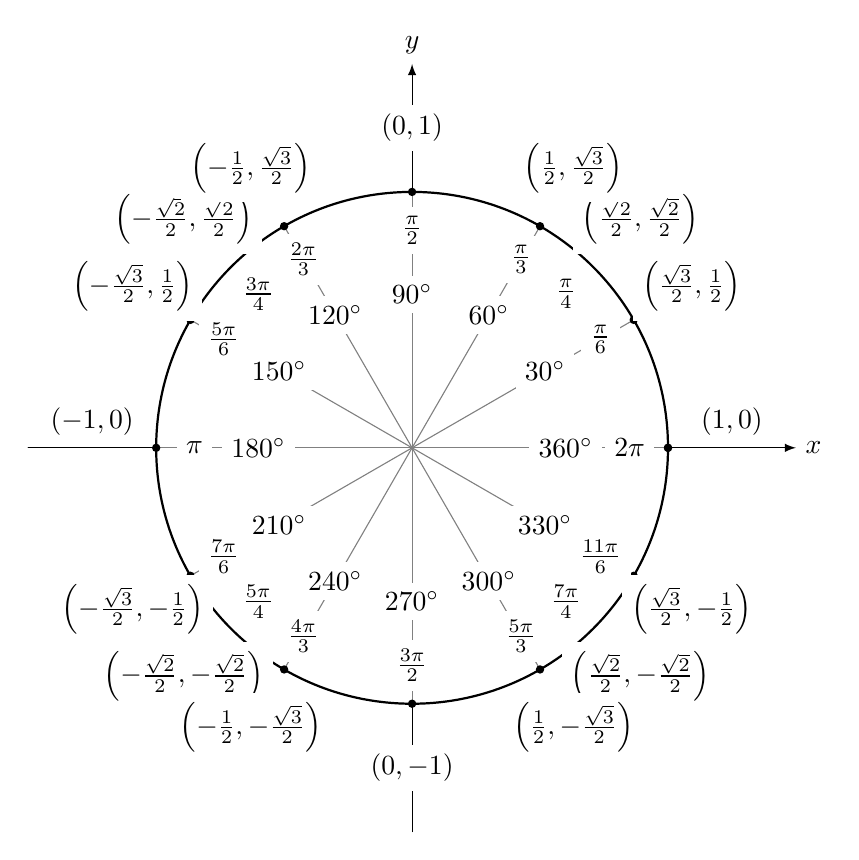
\begin{tikzpicture}[scale=3.25,cap=round,>=latex]         %scale=5,3 % draw the coordinates         
	\draw[->] (-1.5cm,0cm) -- (1.5cm,0cm) node[right,fill=white] {$x$};         
	\draw[->] (0cm,-1.5cm) -- (0cm,1.5cm) node[above,fill=white] {$y$};
        % draw the unit circle         
	\draw[thick] (0cm,0cm) circle(1cm);
    \foreach \x in {0,30,...,360} {                 % lines from center to point                 
			\draw[gray] (0cm,0cm) -- (\x:1cm);                 % dots at each point                 
			\filldraw[black] (\x:1cm) circle(0.4pt);                 % draw each angle in degrees                 
			\draw (\x:0.6cm) node[fill=white] {$\x^\circ$};         
			}
        % draw each angle in radians         
	\foreach \x/\xtext in {
		30/\frac{\pi}{6},             
		45/\frac{\pi}{4},             
		60/\frac{\pi}{3},             			
		90/\frac{\pi}{2},             
		120/\frac{2\pi}{3},             
		135/\frac{3\pi}{4},             
		150/\frac{5\pi}{6},             
		180/\pi,             	
		210/\frac{7\pi}{6},             
		225/\frac{5\pi}{4},             
		240/\frac{4\pi}{3},             
		270/\frac{3\pi}{2},             			
		300/\frac{5\pi}{3},             		
		315/\frac{7\pi}{4},            
		330/\frac{11\pi}{6},             
		360/2\pi}                 
			\draw (\x:0.85cm) node[fill=white] {$\xtext$};
	\foreach \x/\xtext/\y in {             % the coordinates for the first quadrant             
		30/\frac{\sqrt{3}}{2}/\frac{1}{2},             			
		45/\frac{\sqrt{2}}{2}/\frac{\sqrt{2}}{2},             
		60/\frac{1}{2}/\frac{\sqrt{3}}{2},             % the coordinates for the second quadrant             
		150/-\frac{\sqrt{3}}{2}/\frac{1}{2},             
		135/-\frac{\sqrt{2}}{2}/\frac{\sqrt{2}}{2},             			
		120/-\frac{1}{2}/\frac{\sqrt{3}}{2},             % the coordinates for the third quadrant             
		210/-\frac{\sqrt{3}}{2}/-\frac{1}{2},             
		225/-\frac{\sqrt{2}}{2}/-\frac{\sqrt{2}}{2},             
		240/-\frac{1}{2}/-\frac{\sqrt{3}}{2},             % the coordinates for the fourth quadrant             
		330/\frac{\sqrt{3}}{2}/-\frac{1}{2},             				
		315/\frac{\sqrt{2}}{2}/-\frac{\sqrt{2}}{2},             
		300/\frac{1}{2}/-\frac{\sqrt{3}}{2}}                 
			\draw (\x:1.261cm) node[fill=white] {$\left(\xtext,\y\right)$};
        % draw the horizontal and vertical coordinates         % the placement is better this way         
	\draw (-1.25cm,0cm) node[above=1pt] {$(-1,0)$}               
		  (1.25cm,0cm)  node[above=1pt] {$(1,0)$}               
		  (0cm,-1.25cm) node[fill=white] {$(0,-1)$}               
          (0cm,1.25cm)  node[fill=white] {$(0,1)$};     
\end{tikzpicture}

\end{multicols}

\textbf{Trigonometric Substitution Identities}
\begin{enumerate}
\item $a^{2}-x^{2}\rightarrow a^{2}\cos^{2}\theta$ where $x=a\sin\theta$
\item $a^{2}+x^{2}\rightarrow a^{2}\sec^{2}\theta$ where $x=a\sin\theta$
\item $x^{2}-a^{2}\rightarrow a^{2}\tan^{2}\theta$ where $x=a\sec\theta$
\end{enumerate}
\textbf{Pythagorean Identity}
$\sin^{2}\theta+\cos^{2}\theta=1$
\textbf{Half-Angle Formulas }
$\cos^{2}\theta=\frac{1+\cos2\theta}{2}$; ~~$\sin^{2}\theta=\frac{1-\cos2\theta}{2}$
\textbf{Double-Angle Identities}
$\sin2\theta=2\sin\theta\cos\theta$;~~$\cos2\theta=2\cos^{2}\theta-1$
\end{document}
